\documentclass[1p]{elsarticle_modified}
%\bibliographystyle{elsarticle-num}

%\usepackage[colorlinks]{hyperref}
%\usepackage{abbrmath_seonhwa} %\Abb, \Ascr, \Acal ,\Abf, \Afrak
\usepackage{amsfonts}
\usepackage{amssymb}
\usepackage{amsmath}
\usepackage{amsthm}
\usepackage{scalefnt}
\usepackage{amsbsy}
\usepackage{kotex}
\usepackage{caption}
\usepackage{subfig}
\usepackage{color}
\usepackage{graphicx}
\usepackage{xcolor} %% white, black, red, green, blue, cyan, magenta, yellow
\usepackage{float}
\usepackage{setspace}
\usepackage{hyperref}

\usepackage{tikz}
\usetikzlibrary{arrows}

\usepackage{multirow}
\usepackage{array} % fixed length table
\usepackage{hhline}

%%%%%%%%%%%%%%%%%%%%%
\makeatletter
\renewcommand*\env@matrix[1][\arraystretch]{%
	\edef\arraystretch{#1}%
	\hskip -\arraycolsep
	\let\@ifnextchar\new@ifnextchar
	\array{*\c@MaxMatrixCols c}}
\makeatother %https://tex.stackexchange.com/questions/14071/how-can-i-increase-the-line-spacing-in-a-matrix
%%%%%%%%%%%%%%%

\usepackage[normalem]{ulem}

\newcommand{\msout}[1]{\ifmmode\text{\sout{\ensuremath{#1}}}\else\sout{#1}\fi}
%SOURCE: \msout is \stkout macro in https://tex.stackexchange.com/questions/20609/strikeout-in-math-mode

\newcommand{\cancel}[1]{
	\ifmmode
	{\color{red}\msout{#1}}
	\else
	{\color{red}\sout{#1}}
	\fi
}

\newcommand{\add}[1]{
	{\color{blue}\uwave{#1}}
}

\newcommand{\replace}[2]{
	\ifmmode
	{\color{red}\msout{#1}}{\color{blue}\uwave{#2}}
	\else
	{\color{red}\sout{#1}}{\color{blue}\uwave{#2}}
	\fi
}

\newcommand{\Sol}{\mathcal{S}} %segment
\newcommand{\D}{D} %diagram
\newcommand{\A}{\mathcal{A}} %arc


%%%%%%%%%%%%%%%%%%%%%%%%%%%%%5 test

\def\sl{\operatorname{\textup{SL}}(2,\Cbb)}
\def\psl{\operatorname{\textup{PSL}}(2,\Cbb)}
\def\quan{\mkern 1mu \triangleright \mkern 1mu}

\theoremstyle{definition}
\newtheorem{thm}{Theorem}[section]
\newtheorem{prop}[thm]{Proposition}
\newtheorem{lem}[thm]{Lemma}
\newtheorem{ques}[thm]{Question}
\newtheorem{cor}[thm]{Corollary}
\newtheorem{defn}[thm]{Definition}
\newtheorem{exam}[thm]{Example}
\newtheorem{rmk}[thm]{Remark}
\newtheorem{alg}[thm]{Algorithm}

\newcommand{\I}{\sqrt{-1}}
\begin{document}

%\begin{frontmatter}
%
%\title{Boundary parabolic representations of knots up to 8 crossings}
%
%%% Group authors per affiliation:
%\author{Yunhi Cho} 
%\address{Department of Mathematics, University of Seoul, Seoul, Korea}
%\ead{yhcho@uos.ac.kr}
%
%
%\author{Seonhwa Kim} %\fnref{s_kim}}
%\address{Center for Geometry and Physics, Institute for Basic Science, Pohang, 37673, Korea}
%\ead{ryeona17@ibs.re.kr}
%
%\author{Hyuk Kim}
%\address{Department of Mathematical Sciences, Seoul National University, Seoul 08826, Korea}
%\ead{hyukkim@snu.ac.kr}
%
%\author{Seokbeom Yoon}
%\address{Department of Mathematical Sciences, Seoul National University, Seoul, 08826,  Korea}
%\ead{sbyoon15@snu.ac.kr}
%
%\begin{abstract}
%We find all boundary parabolic representation of knots up to 8 crossings.
%
%\end{abstract}
%\begin{keyword}
%    \MSC[2010] 57M25 
%\end{keyword}
%
%\end{frontmatter}

%\linenumbers
%\tableofcontents
%
\newcommand\colored[1]{\textcolor{white}{\rule[-0.35ex]{0.8em}{1.4ex}}\kern-0.8em\color{red} #1}%
%\newcommand\colored[1]{\textcolor{white}{ #1}\kern-2.17ex	\textcolor{white}{ #1}\kern-1.81ex	\textcolor{white}{ #1}\kern-2.15ex\color{red}#1	}

{\Large $\underline{12n_{0045}~(K12n_{0045})}$}

\setlength{\tabcolsep}{10pt}
\renewcommand{\arraystretch}{1.6}
\vspace{1cm}\begin{tabular}{m{100pt}>{\centering\arraybackslash}m{274pt}}
\multirow{5}{120pt}{
	\centering
	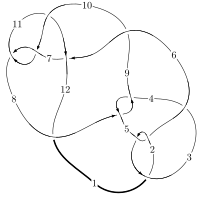
\includegraphics[width=112pt]{../../../GIT/diagram.site/Diagrams/png/2134_12n_0045.png}\\
\ \ \ A knot diagram\footnotemark}&
\allowdisplaybreaks
\textbf{Linearized knot diagam} \\
\cline{2-2}
 &
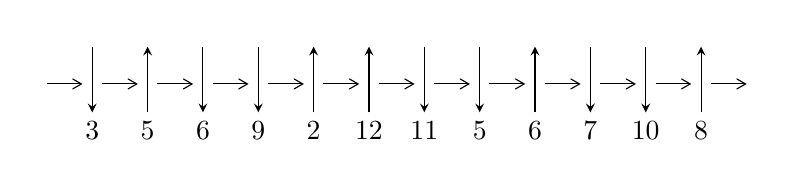
\begin{tikzpicture}[x=20pt, y=17pt]
	% nodes
	\node (C0) at (0, 0) {};
	\node (C1) at (1, 0) {};
	\node (C1U) at (1, +1) {};
	\node (C1D) at (1, -1) {3};

	\node (C2) at (2, 0) {};
	\node (C2U) at (2, +1) {};
	\node (C2D) at (2, -1) {5};

	\node (C3) at (3, 0) {};
	\node (C3U) at (3, +1) {};
	\node (C3D) at (3, -1) {6};

	\node (C4) at (4, 0) {};
	\node (C4U) at (4, +1) {};
	\node (C4D) at (4, -1) {9};

	\node (C5) at (5, 0) {};
	\node (C5U) at (5, +1) {};
	\node (C5D) at (5, -1) {2};

	\node (C6) at (6, 0) {};
	\node (C6U) at (6, +1) {};
	\node (C6D) at (6, -1) {12};

	\node (C7) at (7, 0) {};
	\node (C7U) at (7, +1) {};
	\node (C7D) at (7, -1) {11};

	\node (C8) at (8, 0) {};
	\node (C8U) at (8, +1) {};
	\node (C8D) at (8, -1) {5};

	\node (C9) at (9, 0) {};
	\node (C9U) at (9, +1) {};
	\node (C9D) at (9, -1) {6};

	\node (C10) at (10, 0) {};
	\node (C10U) at (10, +1) {};
	\node (C10D) at (10, -1) {7};

	\node (C11) at (11, 0) {};
	\node (C11U) at (11, +1) {};
	\node (C11D) at (11, -1) {10};

	\node (C12) at (12, 0) {};
	\node (C12U) at (12, +1) {};
	\node (C12D) at (12, -1) {8};
	\node (C13) at (13, 0) {};

	% arrows
	\draw[->,>={angle 60}]
	(C0) edge (C1) (C1) edge (C2) (C2) edge (C3) (C3) edge (C4) (C4) edge (C5) (C5) edge (C6) (C6) edge (C7) (C7) edge (C8) (C8) edge (C9) (C9) edge (C10) (C10) edge (C11) (C11) edge (C12) (C12) edge (C13) ;	\draw[->,>=stealth]
	(C1U) edge (C1D) (C2D) edge (C2U) (C3U) edge (C3D) (C4U) edge (C4D) (C5D) edge (C5U) (C6D) edge (C6U) (C7U) edge (C7D) (C8U) edge (C8D) (C9D) edge (C9U) (C10U) edge (C10D) (C11U) edge (C11D) (C12D) edge (C12U) ;
	\end{tikzpicture} \\
\hhline{~~} \\& 
\textbf{Solving Sequence} \\ \cline{2-2} 
 &
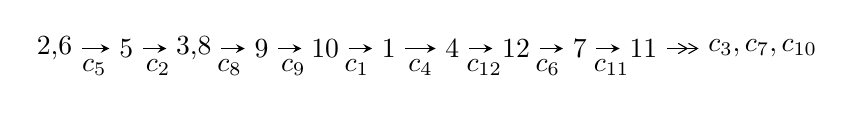
\begin{tikzpicture}[x=23pt, y=7pt]
	% node
	\node (A0) at (-1/8, 0) {2,6};
	\node (A1) at (1, 0) {5};
	\node (A2) at (33/16, 0) {3,8};
	\node (A3) at (25/8, 0) {9};
	\node (A4) at (33/8, 0) {10};
	\node (A5) at (41/8, 0) {1};
	\node (A6) at (49/8, 0) {4};
	\node (A7) at (57/8, 0) {12};
	\node (A8) at (65/8, 0) {7};
	\node (A9) at (73/8, 0) {11};
	\node (C1) at (1/2, -1) {$c_{5}$};
	\node (C2) at (3/2, -1) {$c_{2}$};
	\node (C3) at (21/8, -1) {$c_{8}$};
	\node (C4) at (29/8, -1) {$c_{9}$};
	\node (C5) at (37/8, -1) {$c_{1}$};
	\node (C6) at (45/8, -1) {$c_{4}$};
	\node (C7) at (53/8, -1) {$c_{12}$};
	\node (C8) at (61/8, -1) {$c_{6}$};
	\node (C9) at (69/8, -1) {$c_{11}$};
	\node (A10) at (11, 0) {$c_{3},c_{7},c_{10}$};

	% edge
	\draw[->,>=stealth]	
	(A0) edge (A1) (A1) edge (A2) (A2) edge (A3) (A3) edge (A4) (A4) edge (A5) (A5) edge (A6) (A6) edge (A7) (A7) edge (A8) (A8) edge (A9) ;
	\draw[->>,>={angle 60}]	
	(A9) edge (A10);
\end{tikzpicture} \\ 

\end{tabular} \\

\footnotetext{
The image of knot diagram is generated by the software ``\textbf{Draw programme}" developed by Andrew Bartholomew(\url{http://www.layer8.co.uk/maths/draw/index.htm\#Running-draw}), where we modified some parts for our purpose(\url{https://github.com/CATsTAILs/LinksPainter}).
}\phantom \\ \newline 
\centering \textbf{Ideals for irreducible components\footnotemark of $X_{\text{par}}$} 
 
\begin{align*}
I^u_{1}&=\langle 
-148 u^{29}-963 u^{28}+\cdots+32 b-233,\;-153 u^{29}-960 u^{28}+\cdots+32 a-98,\;u^{30}+7 u^{29}+\cdots+7 u+1\rangle \\
I^u_{2}&=\langle 
- a u+b+a,\;a^6+a^5 u- a^4 u+a^4+2 a^3- a u+a+1,\;u^2- u+1\rangle \\
\\
\end{align*}
\raggedright * 2 irreducible components of $\dim_{\mathbb{C}}=0$, with total 42 representations.\\
\footnotetext{All coefficients of polynomials are rational numbers. But the coefficients are sometimes approximated in decimal forms when there is not enough margin.}
\newpage
\renewcommand{\arraystretch}{1}
\centering \section*{I. $I^u_{1}= \langle -148 u^{29}-963 u^{28}+\cdots+32 b-233,\;-153 u^{29}-960 u^{28}+\cdots+32 a-98,\;u^{30}+7 u^{29}+\cdots+7 u+1 \rangle$}
\flushleft \textbf{(i) Arc colorings}\\
\begin{tabular}{m{7pt} m{180pt} m{7pt} m{180pt} }
\flushright $a_{2}=$&$\begin{pmatrix}0\\u\end{pmatrix}$ \\
\flushright $a_{6}=$&$\begin{pmatrix}1\\0\end{pmatrix}$ \\
\flushright $a_{5}=$&$\begin{pmatrix}1\\u^2\end{pmatrix}$ \\
\flushright $a_{3}=$&$\begin{pmatrix}u\\u^3+u\end{pmatrix}$ \\
\flushright $a_{8}=$&$\begin{pmatrix}4.78125 u^{29}+30 u^{28}+\cdots+28.9688 u+3.06250\\4.62500 u^{29}+30.0938 u^{28}+\cdots+43.3750 u+7.28125\end{pmatrix}$ \\
\flushright $a_{9}=$&$\begin{pmatrix}1.90625 u^{29}+11.6875 u^{28}+\cdots+5.09375 u-0.750000\\3.56250 u^{29}+23.0313 u^{28}+\cdots+33.5625 u+5.46875\end{pmatrix}$ \\
\flushright $a_{10}=$&$\begin{pmatrix}5.46875 u^{29}+34.7188 u^{28}+\cdots+38.6563 u+4.71875\\3.56250 u^{29}+23.0313 u^{28}+\cdots+33.5625 u+5.46875\end{pmatrix}$ \\
\flushright $a_{1}=$&$\begin{pmatrix}u^3\\u^5+u^3+u\end{pmatrix}$ \\
\flushright $a_{4}=$&$\begin{pmatrix}- u^3\\u^3+u\end{pmatrix}$ \\
\flushright $a_{12}=$&$\begin{pmatrix}-0.0312500 u^{28}-0.187500 u^{27}+\cdots-2.18750 u+0.968750\\0.0312500 u^{29}+0.218750 u^{28}+\cdots+0.218750 u+0.0312500\end{pmatrix}$ \\
\flushright $a_{7}=$&$\begin{pmatrix}-\frac{9}{32} u^{29}-2 u^{28}+\cdots-\frac{81}{32} u+\frac{5}{8}\\0.281250 u^{29}+1.71875 u^{28}+\cdots+0.531250 u+0.0312500\end{pmatrix}$ \\
\flushright $a_{11}=$&$\begin{pmatrix}\frac{9}{32} u^{28}+\frac{27}{16} u^{27}+\cdots+2 u+\frac{11}{32}\\-0.281250 u^{29}-1.65625 u^{28}+\cdots+0.843750 u+0.0312500\end{pmatrix}$\\&\end{tabular}
\flushleft \textbf{(ii) Obstruction class $= -1$}\\~\\
\flushleft \textbf{(iii) Cusp Shapes $= \frac{45}{4} u^{29}+\frac{1169}{16} u^{28}+\cdots+103 u+\frac{99}{8}$}\\~\\
\newpage\renewcommand{\arraystretch}{1}
\flushleft \textbf{(iv) u-Polynomials at the component}\newline \\
\begin{tabular}{m{50pt}|m{274pt}}
Crossings & \hspace{64pt}u-Polynomials at each crossing \\
\hline $$\begin{aligned}c_{1}\end{aligned}$$&$\begin{aligned}
&u^{30}+3 u^{29}+\cdots+3 u+1
\end{aligned}$\\
\hline $$\begin{aligned}c_{2},c_{5}\end{aligned}$$&$\begin{aligned}
&u^{30}+7 u^{29}+\cdots+7 u+1
\end{aligned}$\\
\hline $$\begin{aligned}c_{3}\end{aligned}$$&$\begin{aligned}
&u^{30}-7 u^{29}+\cdots+123187 u+9881
\end{aligned}$\\
\hline $$\begin{aligned}c_{4},c_{8}\end{aligned}$$&$\begin{aligned}
&u^{30}+u^{29}+\cdots+8192 u+4096
\end{aligned}$\\
\hline $$\begin{aligned}c_{6}\end{aligned}$$&$\begin{aligned}
&u^{30}+9 u^{29}+\cdots+57 u+17
\end{aligned}$\\
\hline $$\begin{aligned}c_{7},c_{10}\end{aligned}$$&$\begin{aligned}
&u^{30}+3 u^{29}+\cdots+u+1
\end{aligned}$\\
\hline $$\begin{aligned}c_{9},c_{12}\end{aligned}$$&$\begin{aligned}
&u^{30}-3 u^{29}+\cdots-3 u+1
\end{aligned}$\\
\hline $$\begin{aligned}c_{11}\end{aligned}$$&$\begin{aligned}
&u^{30}+13 u^{29}+\cdots-7 u+1
\end{aligned}$\\
\hline
\end{tabular}\\~\\
\newpage\renewcommand{\arraystretch}{1}
\flushleft \textbf{(v) Riley Polynomials at the component}\newline \\
\begin{tabular}{m{50pt}|m{274pt}}
Crossings & \hspace{64pt}Riley Polynomials at each crossing \\
\hline $$\begin{aligned}c_{1}\end{aligned}$$&$\begin{aligned}
&y^{30}+55 y^{29}+\cdots+63 y+1
\end{aligned}$\\
\hline $$\begin{aligned}c_{2},c_{5}\end{aligned}$$&$\begin{aligned}
&y^{30}+3 y^{29}+\cdots+3 y+1
\end{aligned}$\\
\hline $$\begin{aligned}c_{3}\end{aligned}$$&$\begin{aligned}
&y^{30}+107 y^{29}+\cdots+1844116003 y+97634161
\end{aligned}$\\
\hline $$\begin{aligned}c_{4},c_{8}\end{aligned}$$&$\begin{aligned}
&y^{30}+65 y^{29}+\cdots+161480704 y^2+16777216
\end{aligned}$\\
\hline $$\begin{aligned}c_{6}\end{aligned}$$&$\begin{aligned}
&y^{30}-9 y^{29}+\cdots+2531 y+289
\end{aligned}$\\
\hline $$\begin{aligned}c_{7},c_{10}\end{aligned}$$&$\begin{aligned}
&y^{30}-13 y^{29}+\cdots+7 y+1
\end{aligned}$\\
\hline $$\begin{aligned}c_{9},c_{12}\end{aligned}$$&$\begin{aligned}
&y^{30}-53 y^{29}+\cdots+7 y+1
\end{aligned}$\\
\hline $$\begin{aligned}c_{11}\end{aligned}$$&$\begin{aligned}
&y^{30}+11 y^{29}+\cdots-89 y+1
\end{aligned}$\\
\hline
\end{tabular}\\~\\
\newpage\flushleft \textbf{(vi) Complex Volumes and Cusp Shapes}
$$\begin{array}{c|c|c}  
\text{Solutions to }I^u_{1}& \I (\text{vol} + \sqrt{-1}CS) & \text{Cusp shape}\\
 \hline 
\begin{aligned}
u &= \phantom{-}0.156149 + 0.923590 I \\
a &= \phantom{-}1.55521 - 0.59601 I \\
b &= -0.641878 + 0.220216 I\end{aligned}
 & -2.03388 + 4.90769 I & -5.49958 - 7.49846 I \\ \hline\begin{aligned}
u &= \phantom{-}0.156149 - 0.923590 I \\
a &= \phantom{-}1.55521 + 0.59601 I \\
b &= -0.641878 - 0.220216 I\end{aligned}
 & -2.03388 - 4.90769 I & -5.49958 + 7.49846 I \\ \hline\begin{aligned}
u &= \phantom{-}0.399490 + 0.989549 I \\
a &= -0.655955 + 0.923964 I \\
b &= -0.207702 - 0.507122 I\end{aligned}
 & -0.76957 + 1.31164 I & \phantom{-}0.008085 - 1.158902 I \\ \hline\begin{aligned}
u &= \phantom{-}0.399490 - 0.989549 I \\
a &= -0.655955 - 0.923964 I \\
b &= -0.207702 + 0.507122 I\end{aligned}
 & -0.76957 - 1.31164 I & \phantom{-}0.008085 + 1.158902 I \\ \hline\begin{aligned}
u &= \phantom{-}0.918172 + 0.122403 I \\
a &= -0.292882 + 0.357499 I \\
b &= -0.60497 + 1.73623 I\end{aligned}
 & \phantom{-}2.37348 + 2.46946 I & \phantom{-}2.98715 - 3.45316 I \\ \hline\begin{aligned}
u &= \phantom{-}0.918172 - 0.122403 I \\
a &= -0.292882 - 0.357499 I \\
b &= -0.60497 - 1.73623 I\end{aligned}
 & \phantom{-}2.37348 - 2.46946 I & \phantom{-}2.98715 + 3.45316 I \\ \hline\begin{aligned}
u &= \phantom{-}0.780975 + 0.876399 I \\
a &= -1.049250 - 0.803341 I \\
b &= -0.003320 - 1.369010 I\end{aligned}
 & \phantom{-}1.59076 + 0.61155 I & \phantom{-}0.819771 + 0.666887 I \\ \hline\begin{aligned}
u &= \phantom{-}0.780975 - 0.876399 I \\
a &= -1.049250 + 0.803341 I \\
b &= -0.003320 + 1.369010 I\end{aligned}
 & \phantom{-}1.59076 - 0.61155 I & \phantom{-}0.819771 - 0.666887 I \\ \hline\begin{aligned}
u &= \phantom{-}0.362356 + 0.695450 I \\
a &= -0.993697 - 0.057570 I \\
b &= -0.0321747 + 0.0227484 I\end{aligned}
 & -0.194740 + 1.399730 I & -2.02435 - 4.86797 I \\ \hline\begin{aligned}
u &= \phantom{-}0.362356 - 0.695450 I \\
a &= -0.993697 + 0.057570 I \\
b &= -0.0321747 - 0.0227484 I\end{aligned}
 & -0.194740 - 1.399730 I & -2.02435 + 4.86797 I\\
 \hline 
 \end{array}$$\newpage$$\begin{array}{c|c|c}  
\text{Solutions to }I^u_{1}& \I (\text{vol} + \sqrt{-1}CS) & \text{Cusp shape}\\
 \hline 
\begin{aligned}
u &= \phantom{-}0.724731 + 1.015800 I \\
a &= \phantom{-}0.79644 + 1.28595 I \\
b &= -1.11851 + 1.13827 I\end{aligned}
 & \phantom{-}1.10886 + 5.31866 I & -0.13308 - 5.18400 I \\ \hline\begin{aligned}
u &= \phantom{-}0.724731 - 1.015800 I \\
a &= \phantom{-}0.79644 - 1.28595 I \\
b &= -1.11851 - 1.13827 I\end{aligned}
 & \phantom{-}1.10886 - 5.31866 I & -0.13308 + 5.18400 I \\ \hline\begin{aligned}
u &= -0.624839 + 0.318859 I \\
a &= -1.57129 - 0.30420 I \\
b &= -1.44565 + 0.98598 I\end{aligned}
 & \phantom{-}0.78177 - 6.39042 I & -0.72567 + 4.22016 I \\ \hline\begin{aligned}
u &= -0.624839 - 0.318859 I \\
a &= -1.57129 + 0.30420 I \\
b &= -1.44565 - 0.98598 I\end{aligned}
 & \phantom{-}0.78177 + 6.39042 I & -0.72567 - 4.22016 I \\ \hline\begin{aligned}
u &= \phantom{-}0.021362 + 0.665268 I \\
a &= \phantom{-}1.74798 + 0.18763 I \\
b &= -0.284692 - 0.540613 I\end{aligned}
 & -2.74789 - 1.44408 I & -8.12661 + 0.68826 I \\ \hline\begin{aligned}
u &= \phantom{-}0.021362 - 0.665268 I \\
a &= \phantom{-}1.74798 - 0.18763 I \\
b &= -0.284692 + 0.540613 I\end{aligned}
 & -2.74789 + 1.44408 I & -8.12661 - 0.68826 I \\ \hline\begin{aligned}
u &= -0.626826 + 0.181498 I \\
a &= \phantom{-}1.68869 + 0.16006 I \\
b &= \phantom{-}1.59366 - 0.59325 I\end{aligned}
 & \phantom{-}2.71723 - 1.30741 I & \phantom{-}2.25892 + 0.04222 I \\ \hline\begin{aligned}
u &= -0.626826 - 0.181498 I \\
a &= \phantom{-}1.68869 - 0.16006 I \\
b &= \phantom{-}1.59366 + 0.59325 I\end{aligned}
 & \phantom{-}2.71723 + 1.30741 I & \phantom{-}2.25892 - 0.04222 I \\ \hline\begin{aligned}
u &= -1.03232 + 1.03051 I \\
a &= -1.33615 - 1.25080 I \\
b &= -2.95729 + 0.40290 I\end{aligned}
 & \phantom{-}11.18100 - 3.78919 I & -2.00000 + 1.99020 I \\ \hline\begin{aligned}
u &= -1.03232 - 1.03051 I \\
a &= -1.33615 + 1.25080 I \\
b &= -2.95729 - 0.40290 I\end{aligned}
 & \phantom{-}11.18100 + 3.78919 I & -2.00000 - 1.99020 I\\
 \hline 
 \end{array}$$\newpage$$\begin{array}{c|c|c}  
\text{Solutions to }I^u_{1}& \I (\text{vol} + \sqrt{-1}CS) & \text{Cusp shape}\\
 \hline 
\begin{aligned}
u &= -1.13894 + 0.98249 I \\
a &= -0.85062 - 1.72090 I \\
b &= -4.00129 - 1.44921 I\end{aligned}
 & \phantom{-}16.0192 + 4.0819 I & \phantom{-0.000000 } 0 \\ \hline\begin{aligned}
u &= -1.13894 - 0.98249 I \\
a &= -0.85062 + 1.72090 I \\
b &= -4.00129 + 1.44921 I\end{aligned}
 & \phantom{-}16.0192 - 4.0819 I & \phantom{-0.000000 } 0 \\ \hline\begin{aligned}
u &= -1.00742 + 1.12472 I \\
a &= -1.90712 - 1.30827 I \\
b &= -3.23563 + 2.16136 I\end{aligned}
 & \phantom{-}15.4793 - 11.9246 I & \phantom{-0.000000 -}0. + 6.30873 I \\ \hline\begin{aligned}
u &= -1.00742 - 1.12472 I \\
a &= -1.90712 + 1.30827 I \\
b &= -3.23563 - 2.16136 I\end{aligned}
 & \phantom{-}15.4793 + 11.9246 I & \phantom{-0.000000 } 0. - 6.30873 I \\ \hline\begin{aligned}
u &= -1.12156 + 1.02634 I \\
a &= \phantom{-}1.12316 + 1.72616 I \\
b &= \phantom{-}4.29671 + 0.57523 I\end{aligned}
 & \phantom{-}17.7688 - 1.7617 I & \phantom{-0.000000 } 0 \\ \hline\begin{aligned}
u &= -1.12156 - 1.02634 I \\
a &= \phantom{-}1.12316 - 1.72616 I \\
b &= \phantom{-}4.29671 - 0.57523 I\end{aligned}
 & \phantom{-}17.7688 + 1.7617 I & \phantom{-0.000000 } 0 \\ \hline\begin{aligned}
u &= -1.04184 + 1.10803 I \\
a &= \phantom{-}1.74324 + 1.46487 I \\
b &= \phantom{-}3.74797 - 1.61674 I\end{aligned}
 & \phantom{-}17.4515 - 6.1631 I & \phantom{-0.000000 } 0 \\ \hline\begin{aligned}
u &= -1.04184 - 1.10803 I \\
a &= \phantom{-}1.74324 - 1.46487 I \\
b &= \phantom{-}3.74797 + 1.61674 I\end{aligned}
 & \phantom{-}17.4515 + 6.1631 I & \phantom{-0.000000 } 0 \\ \hline\begin{aligned}
u &= -0.269490 + 0.299415 I \\
a &= -1.99775 - 0.56157 I \\
b &= -0.605235 + 0.631449 I\end{aligned}
 & -1.76892 + 0.41411 I & -5.79951 - 1.41452 I \\ \hline\begin{aligned}
u &= -0.269490 - 0.299415 I \\
a &= -1.99775 + 0.56157 I \\
b &= -0.605235 - 0.631449 I\end{aligned}
 & -1.76892 - 0.41411 I & -5.79951 + 1.41452 I\\
 \hline 
 \end{array}$$\newpage\newpage\renewcommand{\arraystretch}{1}
\centering \section*{II. $I^u_{2}= \langle - a u+b+a,\;a^6+a^5 u- a^4 u+a^4+2 a^3- a u+a+1,\;u^2- u+1 \rangle$}
\flushleft \textbf{(i) Arc colorings}\\
\begin{tabular}{m{7pt} m{180pt} m{7pt} m{180pt} }
\flushright $a_{2}=$&$\begin{pmatrix}0\\u\end{pmatrix}$ \\
\flushright $a_{6}=$&$\begin{pmatrix}1\\0\end{pmatrix}$ \\
\flushright $a_{5}=$&$\begin{pmatrix}1\\u-1\end{pmatrix}$ \\
\flushright $a_{3}=$&$\begin{pmatrix}u\\u-1\end{pmatrix}$ \\
\flushright $a_{8}=$&$\begin{pmatrix}a\\a u- a\end{pmatrix}$ \\
\flushright $a_{9}=$&$\begin{pmatrix}a\\a u- a\end{pmatrix}$ \\
\flushright $a_{10}=$&$\begin{pmatrix}a u\\a u- a\end{pmatrix}$ \\
\flushright $a_{1}=$&$\begin{pmatrix}-1\\0\end{pmatrix}$ \\
\flushright $a_{4}=$&$\begin{pmatrix}1\\u-1\end{pmatrix}$ \\
\flushright $a_{12}=$&$\begin{pmatrix}- a^2 u+a^2-1\\a^2 u\end{pmatrix}$ \\
\flushright $a_{7}=$&$\begin{pmatrix}- a^4+a^2 u+1\\- a^4 u+a^4\end{pmatrix}$ \\
\flushright $a_{11}=$&$\begin{pmatrix}- a^4 u- a^2 u-1\\- a^4 u+a^4\end{pmatrix}$\\&\end{tabular}
\flushleft \textbf{(ii) Obstruction class $= 1$}\\~\\
\flushleft \textbf{(iii) Cusp Shapes $= - a^5 u+a^5-4 a^4 u+4 a^4-2 a^3 u-5 a^2 u+2 a^2-4 a u+2 a-5 u-2$}\\~\\
\newpage\renewcommand{\arraystretch}{1}
\flushleft \textbf{(iv) u-Polynomials at the component}\newline \\
\begin{tabular}{m{50pt}|m{274pt}}
Crossings & \hspace{64pt}u-Polynomials at each crossing \\
\hline $$\begin{aligned}c_{1},c_{3},c_{5}\end{aligned}$$&$\begin{aligned}
&(u^2- u+1)^6
\end{aligned}$\\
\hline $$\begin{aligned}c_{2}\end{aligned}$$&$\begin{aligned}
&(u^2+u+1)^6
\end{aligned}$\\
\hline $$\begin{aligned}c_{4},c_{8}\end{aligned}$$&$\begin{aligned}
&u^{12}
\end{aligned}$\\
\hline $$\begin{aligned}c_{6},c_{11}\end{aligned}$$&$\begin{aligned}
&(u^6+3 u^5+5 u^4+4 u^3+2 u^2+u+1)^2
\end{aligned}$\\
\hline $$\begin{aligned}c_{7},c_{9},c_{12}\end{aligned}$$&$\begin{aligned}
&(u^6+u^5- u^4-2 u^3+u+1)^2
\end{aligned}$\\
\hline $$\begin{aligned}c_{10}\end{aligned}$$&$\begin{aligned}
&(u^6- u^5- u^4+2 u^3- u+1)^2
\end{aligned}$\\
\hline
\end{tabular}\\~\\
\newpage\renewcommand{\arraystretch}{1}
\flushleft \textbf{(v) Riley Polynomials at the component}\newline \\
\begin{tabular}{m{50pt}|m{274pt}}
Crossings & \hspace{64pt}Riley Polynomials at each crossing \\
\hline $$\begin{aligned}c_{1},c_{2},c_{3}\\c_{5}\end{aligned}$$&$\begin{aligned}
&(y^2+y+1)^6
\end{aligned}$\\
\hline $$\begin{aligned}c_{4},c_{8}\end{aligned}$$&$\begin{aligned}
&y^{12}
\end{aligned}$\\
\hline $$\begin{aligned}c_{6},c_{11}\end{aligned}$$&$\begin{aligned}
&(y^6+y^5+5 y^4+6 y^2+3 y+1)^2
\end{aligned}$\\
\hline $$\begin{aligned}c_{7},c_{9},c_{10}\\c_{12}\end{aligned}$$&$\begin{aligned}
&(y^6-3 y^5+5 y^4-4 y^3+2 y^2- y+1)^2
\end{aligned}$\\
\hline
\end{tabular}\\~\\
\newpage\flushleft \textbf{(vi) Complex Volumes and Cusp Shapes}
$$\begin{array}{c|c|c}  
\text{Solutions to }I^u_{2}& \I (\text{vol} + \sqrt{-1}CS) & \text{Cusp shape}\\
 \hline 
\begin{aligned}
u &= \phantom{-}0.500000 + 0.866025 I \\
a &= \phantom{-}0.245150 + 1.015700 I \\
b &= -1.002190 - 0.295542 I\end{aligned}
 & \phantom{-}1.89061 + 1.10558 I & \phantom{-}1.81693 - 2.49433 I \\ \hline\begin{aligned}
u &= \phantom{-}0.500000 + 0.866025 I \\
a &= \phantom{-}0.757043 + 0.720154 I \\
b &= -1.002190 + 0.295542 I\end{aligned}
 & \phantom{-}1.89061 + 2.95419 I & -0.06995 - 4.17815 I \\ \hline\begin{aligned}
u &= \phantom{-}0.500000 + 0.866025 I \\
a &= -0.789622 - 0.038604 I \\
b &= \phantom{-}0.428243 - 0.664531 I\end{aligned}
 & -1.89061 + 1.10558 I & -7.01188 - 1.87706 I \\ \hline\begin{aligned}
u &= \phantom{-}0.500000 + 0.866025 I \\
a &= \phantom{-}0.361379 - 0.703135 I \\
b &= \phantom{-}0.428243 + 0.664531 I\end{aligned}
 & -1.89061 + 2.95419 I & -3.50232 - 4.35344 I \\ \hline\begin{aligned}
u &= \phantom{-}0.500000 + 0.866025 I \\
a &= -1.020870 - 0.650692 I \\
b &= \phantom{-}1.073950 - 0.558752 I\end{aligned}
 & \phantom{-0.000000 } -3.66314 I & -1.09315 + 2.75648 I \\ \hline\begin{aligned}
u &= \phantom{-}0.500000 + 0.866025 I \\
a &= -0.053081 - 1.209440 I \\
b &= \phantom{-}1.073950 + 0.558752 I\end{aligned}
 & \phantom{-0.000000 -}7.72290 I & -4.13964 - 8.90605 I \\ \hline\begin{aligned}
u &= \phantom{-}0.500000 - 0.866025 I \\
a &= \phantom{-}0.245150 - 1.015700 I \\
b &= -1.002190 + 0.295542 I\end{aligned}
 & \phantom{-}1.89061 - 1.10558 I & \phantom{-}1.81693 + 2.49433 I \\ \hline\begin{aligned}
u &= \phantom{-}0.500000 - 0.866025 I \\
a &= \phantom{-}0.757043 - 0.720154 I \\
b &= -1.002190 - 0.295542 I\end{aligned}
 & \phantom{-}1.89061 - 2.95419 I & -0.06995 + 4.17815 I \\ \hline\begin{aligned}
u &= \phantom{-}0.500000 - 0.866025 I \\
a &= -0.789622 + 0.038604 I \\
b &= \phantom{-}0.428243 + 0.664531 I\end{aligned}
 & -1.89061 - 1.10558 I & -7.01188 + 1.87706 I \\ \hline\begin{aligned}
u &= \phantom{-}0.500000 - 0.866025 I \\
a &= \phantom{-}0.361379 + 0.703135 I \\
b &= \phantom{-}0.428243 - 0.664531 I\end{aligned}
 & -1.89061 - 2.95419 I & -3.50232 + 4.35344 I\\
 \hline 
 \end{array}$$\newpage$$\begin{array}{c|c|c}  
\text{Solutions to }I^u_{2}& \I (\text{vol} + \sqrt{-1}CS) & \text{Cusp shape}\\
 \hline 
\begin{aligned}
u &= \phantom{-}0.500000 - 0.866025 I \\
a &= -1.020870 + 0.650692 I \\
b &= \phantom{-}1.073950 + 0.558752 I\end{aligned}
 & \phantom{-0.000000 -}3.66314 I & -1.09315 - 2.75648 I \\ \hline\begin{aligned}
u &= \phantom{-}0.500000 - 0.866025 I \\
a &= -0.053081 + 1.209440 I \\
b &= \phantom{-}1.073950 - 0.558752 I\end{aligned}
 & \phantom{-0.000000 } -7.72290 I & -4.13964 + 8.90605 I\\
 \hline 
 \end{array}$$\newpage
\newpage\renewcommand{\arraystretch}{1}
\centering \section*{ III. u-Polynomials}
\begin{tabular}{m{50pt}|m{274pt}}
Crossings & \hspace{64pt}u-Polynomials at each crossing \\
\hline $$\begin{aligned}c_{1}\end{aligned}$$&$\begin{aligned}
&((u^2- u+1)^6)(u^{30}+3 u^{29}+\cdots+3 u+1)
\end{aligned}$\\
\hline $$\begin{aligned}c_{2}\end{aligned}$$&$\begin{aligned}
&((u^2+u+1)^6)(u^{30}+7 u^{29}+\cdots+7 u+1)
\end{aligned}$\\
\hline $$\begin{aligned}c_{3}\end{aligned}$$&$\begin{aligned}
&((u^2- u+1)^6)(u^{30}-7 u^{29}+\cdots+123187 u+9881)
\end{aligned}$\\
\hline $$\begin{aligned}c_{4},c_{8}\end{aligned}$$&$\begin{aligned}
&u^{12}(u^{30}+u^{29}+\cdots+8192 u+4096)
\end{aligned}$\\
\hline $$\begin{aligned}c_{5}\end{aligned}$$&$\begin{aligned}
&((u^2- u+1)^6)(u^{30}+7 u^{29}+\cdots+7 u+1)
\end{aligned}$\\
\hline $$\begin{aligned}c_{6}\end{aligned}$$&$\begin{aligned}
&((u^6+3 u^5+5 u^4+4 u^3+2 u^2+u+1)^{2})(u^{30}+9 u^{29}+\cdots+57 u+17)
\end{aligned}$\\
\hline $$\begin{aligned}c_{7}\end{aligned}$$&$\begin{aligned}
&((u^6+u^5- u^4-2 u^3+u+1)^2)(u^{30}+3 u^{29}+\cdots+u+1)
\end{aligned}$\\
\hline $$\begin{aligned}c_{9},c_{12}\end{aligned}$$&$\begin{aligned}
&((u^6+u^5- u^4-2 u^3+u+1)^2)(u^{30}-3 u^{29}+\cdots-3 u+1)
\end{aligned}$\\
\hline $$\begin{aligned}c_{10}\end{aligned}$$&$\begin{aligned}
&((u^6- u^5- u^4+2 u^3- u+1)^2)(u^{30}+3 u^{29}+\cdots+u+1)
\end{aligned}$\\
\hline $$\begin{aligned}c_{11}\end{aligned}$$&$\begin{aligned}
&((u^6+3 u^5+5 u^4+4 u^3+2 u^2+u+1)^{2})(u^{30}+13 u^{29}+\cdots-7 u+1)
\end{aligned}$\\
\hline
\end{tabular}\newpage\renewcommand{\arraystretch}{1}
\centering \section*{ IV. Riley Polynomials}
\begin{tabular}{m{50pt}|m{274pt}}
Crossings & \hspace{64pt}Riley Polynomials at each crossing \\
\hline $$\begin{aligned}c_{1}\end{aligned}$$&$\begin{aligned}
&((y^2+y+1)^6)(y^{30}+55 y^{29}+\cdots+63 y+1)
\end{aligned}$\\
\hline $$\begin{aligned}c_{2},c_{5}\end{aligned}$$&$\begin{aligned}
&((y^2+y+1)^6)(y^{30}+3 y^{29}+\cdots+3 y+1)
\end{aligned}$\\
\hline $$\begin{aligned}c_{3}\end{aligned}$$&$\begin{aligned}
&((y^2+y+1)^6)(y^{30}+107 y^{29}+\cdots+1.84412\times10^{9} y+9.76342\times10^{7})
\end{aligned}$\\
\hline $$\begin{aligned}c_{4},c_{8}\end{aligned}$$&$\begin{aligned}
&y^{12}(y^{30}+65 y^{29}+\cdots+1.61481\times10^{8} y^{2}+1.67772\times10^{7})
\end{aligned}$\\
\hline $$\begin{aligned}c_{6}\end{aligned}$$&$\begin{aligned}
&((y^6+y^5+5 y^4+6 y^2+3 y+1)^2)(y^{30}-9 y^{29}+\cdots+2531 y+289)
\end{aligned}$\\
\hline $$\begin{aligned}c_{7},c_{10}\end{aligned}$$&$\begin{aligned}
&((y^6-3 y^5+5 y^4-4 y^3+2 y^2- y+1)^{2})(y^{30}-13 y^{29}+\cdots+7 y+1)
\end{aligned}$\\
\hline $$\begin{aligned}c_{9},c_{12}\end{aligned}$$&$\begin{aligned}
&((y^6-3 y^5+5 y^4-4 y^3+2 y^2- y+1)^{2})(y^{30}-53 y^{29}+\cdots+7 y+1)
\end{aligned}$\\
\hline $$\begin{aligned}c_{11}\end{aligned}$$&$\begin{aligned}
&((y^6+y^5+5 y^4+6 y^2+3 y+1)^2)(y^{30}+11 y^{29}+\cdots-89 y+1)
\end{aligned}$\\
\hline
\end{tabular}
\vskip 2pc
\end{document}